
\subsection{Shared Space træk i Nytorv/Østerågade området}
\label{omrade_sharedspace}
For at få en forståelse af hvordan trafikanterne færdes i Nytorv/Østerågade området, er det vigtigt først at fastlægge, hvilken type område det er. Området har mange træk fra Shared Space, og derfor er det relevant at sammenligne området med dette begreb. 
Tit og ofte anvender man Shared Space i områder, hvor der er et kryds, eller hvor der er et sammenhængende område, for at skabe en slags balance mellem de forskellige trafikantgrupper. ((en kilde))

\begin{figure}[htbp]
   \label{fig:Nytorv}
   \centering
   \begin{adjustbox}{max width=\textwidth}
     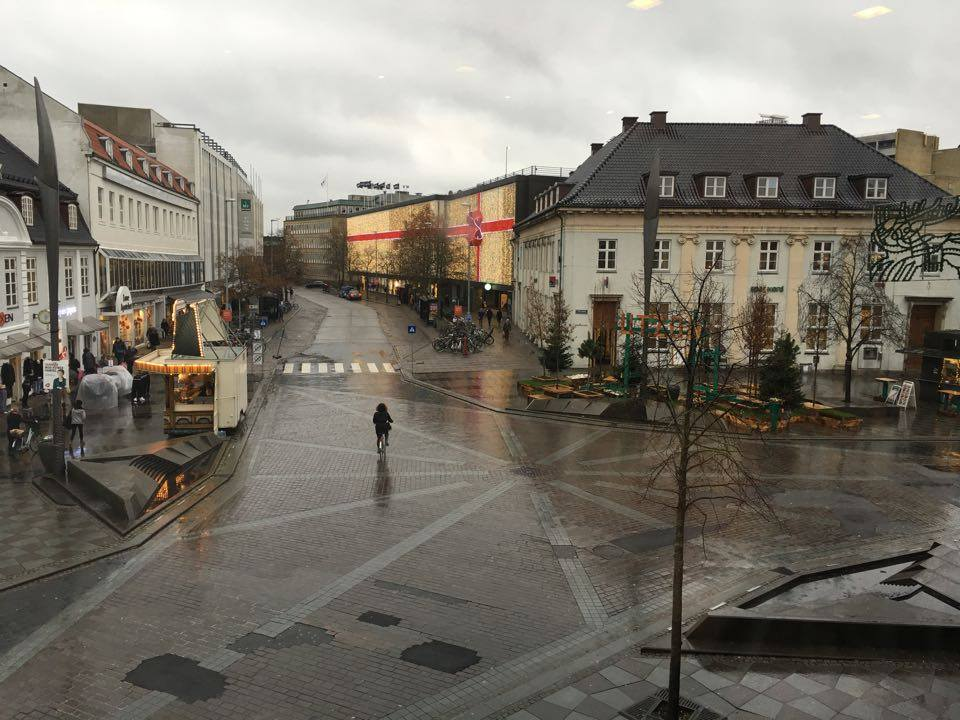
\includegraphics[scale=0.3]{billederogfigur/Nytorvoverblik.jpg}
  \end{adjustbox}
   \caption{Oveblik over Nytorv}
 \end{figure}

Med en balance menes der, at et af formålene med et Shared Space er at ingen af trafikantgrupperne vægtes højere end andre trafikantgrupper. På den måde vil man ikke bryde et sammenhængende område, da man forsøger at kombinere hele områdets funktioner i et. Netop dette princip kan man tydeligt fornemme nede ved Nytorv/Østerågade området. På figur 4.1 kan man se, at området består af et T-kryds, hvor der rundt om er placeret mange shopping faciliteter og caféer. Desuden forbinder området de to gågader, som gør området til et sammenhængende område. Kriterierne for et område, hvor Shared Space kan benyttes, er altså her opfyldt. 
Det er tydeligt, at belægningerne, både på fortov og vej, er meget lig udeseende, hvilket er typisk for et Shared Space område ((kilde)). Der er heller ikke meget afmærkning i form af cykelstier eller kørebaner, som ville have haft til formål at lede trafikanterne. Skiltning, er heller ikke meget brugt og typisk ser man kun et ”E49-, E51- eller E53-skilt” i Shared Space områder, som enten fortæller, om det er en gågade, opholds- og legeområde, eller en fartdæmpet zone, hvor makshastigheden typisk må være 20-30 km/t. Der er altså ikke noget skilt, som decideret er tildelt til Shared Space områder. ((kilde)) Rundt om Nytorv/Østerågade området, er der skiltet med E53-skilte, hvor der er en tilladt makshastighed på 30 km/t. Det kan ses på figur 4.2, som er taget ved Adelgade, lige inden man kommer ind i Nytorv/Østerågade området.

\begin{figure}[htbp]
   \label{fig:Skiltning}
   \centering
   \begin{adjustbox}{max width=\textwidth}
     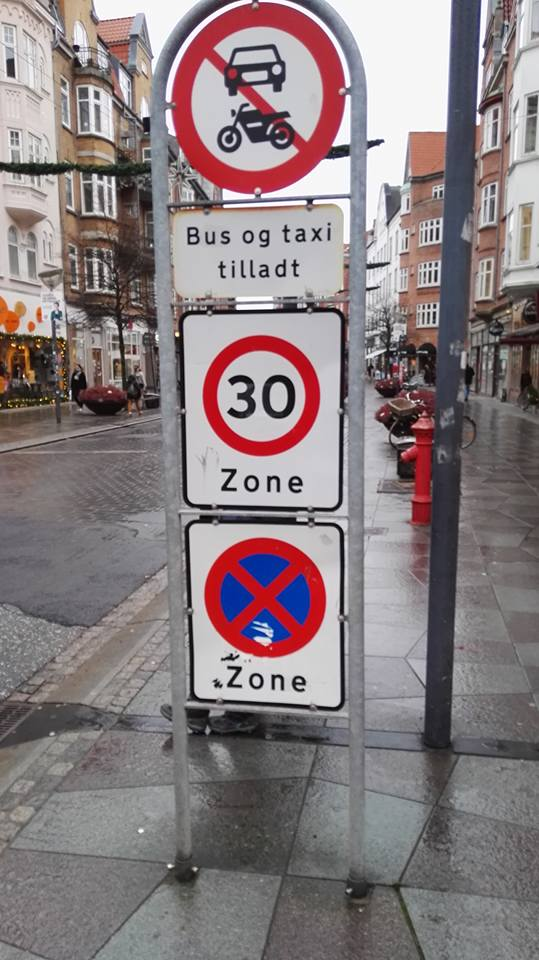
\includegraphics[scale=0.2]{billederogfigur/skiltning.jpg}
  \end{adjustbox}
   \caption{Skiltning rundt om området}
 \end{figure}
\linebreak
I området er der dog en del bustrafik, som ikke anbefales at benytte sig af gennem et Shared Space område. Det er hovedsagligt fordi fokus er på balancen mellem trafikantgrupperne. Busserne vil ofte være nødsaget til at skulle holde tilbage for de mange passerende fodgængere, og det vil kunne forsinke bustrafikken og dermed den kollektive trafik. Dog er der oftest i ruteplanerne taget højde for en sådan forsinkelse, og på korte strækninger vil indflydelsen kunne tænkes at være begrænset. Busserne kræver nogle busstoppesteder, for at passagerer kan stige af og på busserne i området. 

\begin{figure}[htbp]
   \label{fig:Busstoppesteder}
   \centering
   \begin{adjustbox}{max width=\textwidth}
     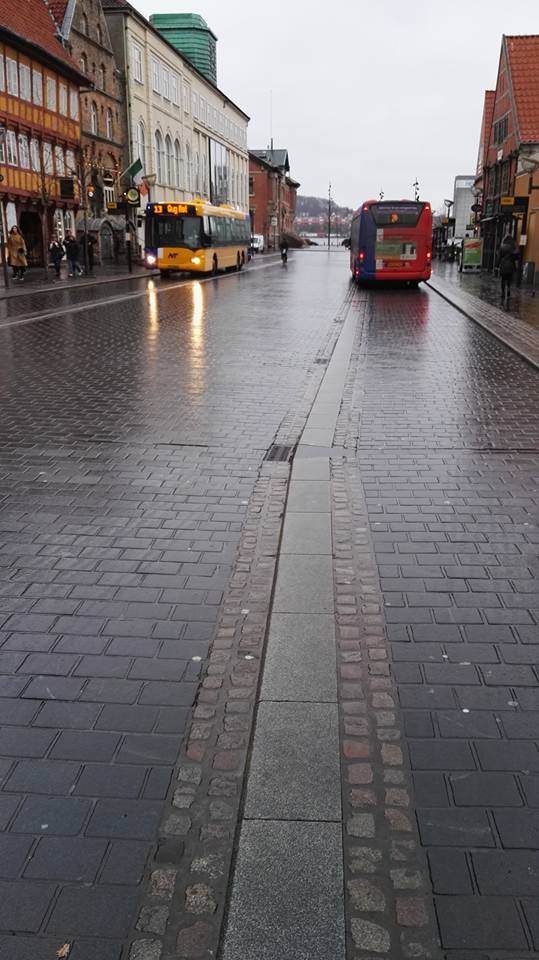
\includegraphics[scale=0.2]{billederogfigur/Busstoppesteder.jpg}
  \end{adjustbox}
   \caption{De to busstoppesteder}
 \end{figure}

På figur 4.3 kan man se de to etablerede busstoppesteder, som er placeret lige efter, hvor Bispensgade udmunder ved Østerågade((henvis til flow kortet)). Placeringen af bustoppestederne er lige udenfor det mest befærdede område, som strækker sig mellem de to gågader og ned ad Nytorv. Placeringen er medvirke til, at det skaber mindst mulige trafikale problemer. Logisk er det også det helt rigtige sted det er placeret, da det reelt set er det eneste sted i området, hvor der er plads til en sådan etablering. 
I et Shared Space område kræves også mange holdepladser til cykler. På Nytorv er der på begge sider af vejen et forholdsvist bredt fortov, som har til formål, at skabe en masse plads, hvor cyklerne kan holde parkeret. Det er en nødvendighed, da der færdes mange cykler i området, og for at de mange cyklister skal kunne benytte sig af de mange shopping faciliteter, kræves der altså nogle holdesteder. ((mangler billede af holdepladser))
Der er altså rigtigt mange træk, som man i området kan observere, minder meget om et Shared Space’ princip, og projektet vil i det næste afsnit undersøge, hvordan området bliver benyttet. 

\subsection{Trafikanternes benyttelse af Nytorv som et Shared Space}
\label{benyttelse_omrade}
Den ens belægning, den manglende afmærkning og de få skilte kan gøre det svært at orientere sig i Nytorv/Østerågade området. Der er meget få retningslinjer og afmærkning til at lede trafikanterne, hvis stort set ingen.

\begin{figure}[htbp]
   \label{fig:Fodfelt}
   \centering
   \begin{adjustbox}{max width=\textwidth}
     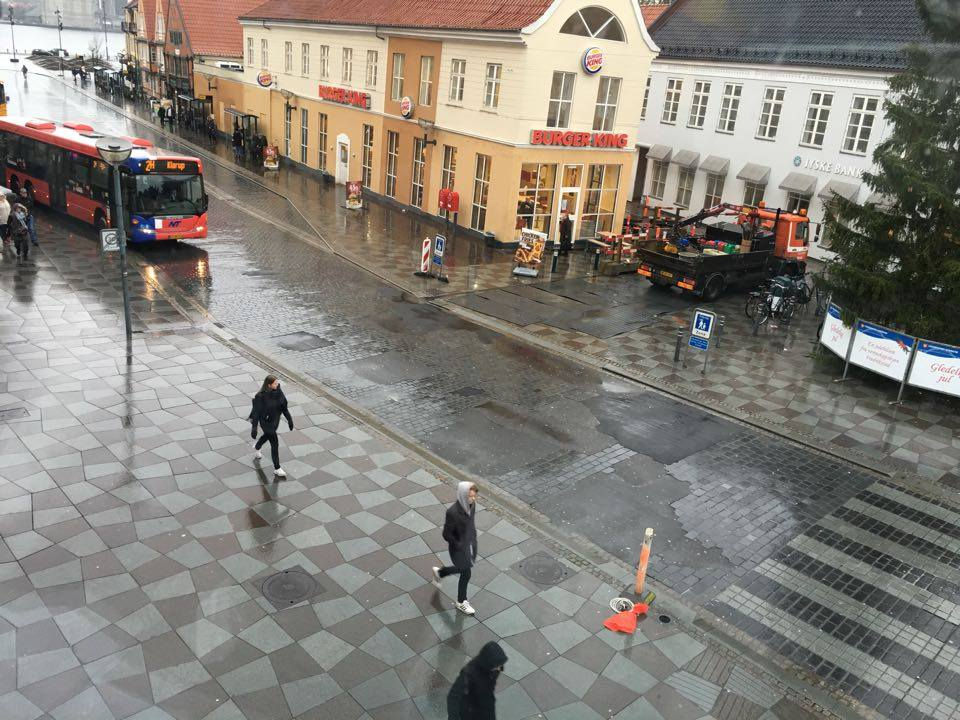
\includegraphics[scale=0.3]{billederogfigur/Fodfelt.jpg}
  \end{adjustbox}
   \caption{Fodgængeroverfeltet}
 \end{figure}

På figur 4.4 kan man se et af de to fodgængerfelter, som er i området. Det er på billedet let nok at se afmærkningerne, da billedet er taget fra et fugleperspektiv. Men en observation af dette område kan bekræfte, at det kan være svært for cyklisterne at se fodgængerfeltet, når de kommer cyklende mod det. Det er især cyklister, som kommer rundt svinget fra Nytorv mod havnen. Svinget kan ses til venstre i billedet på figur 4.1. Der skal her nævnes, at fodgængerfeltet er placeret lige efter svinget, så man kan her forestille sig at figur 4.1 og 4.4 hænger sammen. Det er blandt andet også denne hypotese, at interviewsene senere i rapporten tager lidt udgangspunkt i, hvor trygheden for de passerende fodgængere undersøges. 
Det er dog langt fra alle fodgængerne der benytter sig af fodgængerfelterne. Der er ikke et fast struktureret trafik flow, som man ved andre områder vil kunne observere. Mange fodgængere passere området midt over torvet, som er det torv, der er illustreret på figur 4.1. Cyklisterne agerer også meget uensartet, og det er netop en af sideeffekterne ved et Shared Space område. En undersøgelse af trafik flowet i området, vil blive undersøgt senere i rapporten. Det er her spørgsmålet kommer ind i billedet, om flere retningslinjer vil skabe mere tryghed, eller et uensartet trafik flow er lige så trygt at færdes i. Det er i hvert fald tydeligt, at der er blevet formået at binde området sammen set fra de bløde trafikanters perspektiv. Udelukkelsen af biler har tydeligt præget fordelingen af trafikantgrupper i området, og langt størstedelen er fodgængere og cyklister. Den balancerende virkning mellem de forskellige trafikantgrupper er også tilstede, og det er ikke et område, hvor man vil forvente en masse ulykker. En vurdering af området tyder på, at den indbyrdes respekt overfor hinanden, mellem de forskellige trafikantgrupper, ikke er pålagt af området, men individet selv, netop fordi, at området ikke pålægger det. Shared Space har altså en form for psykologisk effekt, som får trafikanterne til at være opmærksomme på hinanden, og hjælpe hinanden gennem området bedst muligt. Dog er dette ikke et argument for et trygt område at færdes i. Kvalitative interviews vil her være en god måde at undersøge på, om især fodgængerne føler sig trygge, ved at passere området.
De biler, som på trods af forbuddet, vælger at færdes dernede, kører generelt med en lav hastighed. Det samme er at sige om busserne. De opfylder også oftest kravet om en pålagt respekt overfor de bløde trafikanter, og holder tilbage for fodgængeroverfeltet. I forhold til bustrafikken, må det som antaget, forsinke dem en smule, dog begrænset, da det kun er det ene fodgængerfelt, der skal passeres. 
I det næste afsnit vil der blive undersøgt via kvalitative interviews, om fodgængerne føler sig trygge overfor cyklisterne, busserne og bilerne, når de passere fodgængeroverfeltet. Herved også for at få en forståelse af, om den balance Shared Space har til formål, er opfyldt.
